\documentclass[10pt,twocolumn,letterpaper]{article}

\usepackage{iccv}
\usepackage{times}
\usepackage{epsfig}
\usepackage{graphicx}
\usepackage{amsmath}
\usepackage{amssymb}

\usepackage{subfloat}
\usepackage{subfigure}
\usepackage{amsmath}
\usepackage{amssymb}
\usepackage{verbatim}
\usepackage{epsfig}
\usepackage{graphicx}
\usepackage{caption}
\usepackage{enumerate}
% Include other packages here, before hyperref.

% If you comment hyperref and then uncomment it, you should delete
% egpaper.aux before re-running latex.  (Or just hit 'q' on the first latex
% run, let it finish, and you should be clear).
\usepackage[pagebackref=true,breaklinks=true,letterpaper=true,colorlinks,bookmarks=false]{hyperref}

% \iccvfinalcopy % *** Uncomment this line for the final submission

\def\iccvPaperID{****} % *** Enter the ICCV Paper ID here
\def\httilde{\mbox{\tt\raisebox{-.5ex}{\symbol{126}}}}

% Pages are numbered in submission mode, and unnumbered in camera-ready
\ificcvfinal\pagestyle{empty}\fi
\begin{document}

%%%%%%%%% TITLE
\title{What makes an object memorable?}

\author{First Author\\
Institution1\\
Institution1 address\\
{\tt\small firstauthor@i1.org}
% For a paper whose authors are all at the same institution,
% omit the following lines up until the closing ``}''.
% Additional authors and addresses can be added with ``\and'',
% just like the second author.
% To save space, use either the email address or home page, not both
\and
Second Author\\
Institution2\\
First line of institution2 address\\
{\tt\small secondauthor@i2.org}
}

\maketitle
%\thispagestyle{empty}


%%%%%%%%% ABSTRACT
\begin{abstract}
  The ABSTRACT is to be in fully-justified italicized text, at the top
   of the left-hand column, below the author and affiliation
   information. Use the word ``Abstract'' as the title, in 12-point
   Times, boldface type, centered relative to the column, initially
   capitalized. The abstract is to be in 10-point, single-spaced type.
   Leave two blank lines after the Abstract, then begin the main text.
   Look at previous ICCV abstracts to get a feel for style and length.
\end{abstract}

%%%%%%%%% BODY TEXT
\section{Introduction}

Consider the image and it's corresponding objects in Figure \ref{fig:introPhoto}. Even though the person on the right is comparable in size to the left person, he is remembered far less by humans (indicated by their memorability scores of $0.18$ and $0.64$ respectively). People tend to remember the fish in the center and the person on the left, even after $30$ minutes have passed (memorability score $= 0.64$). Interestingly, despite vibrant colors and considerable size, the boat is also remembered far less by humans (memorability $= 0.18$).


\begin{figure}[t]
\centering
\subfigure{\centering 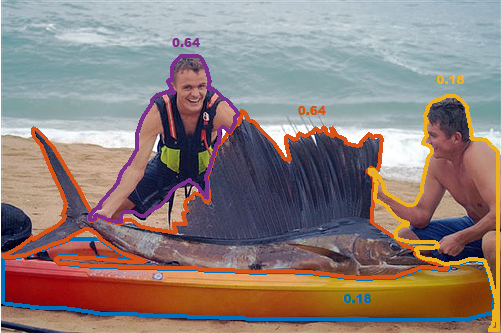
\includegraphics[width=0.2\textwidth]{figures/introduction/intro.png}}
\subfigure{\centering 
\includegraphics[width=0.2\textwidth]{figures/introduction/113.png}}
\vspace{-5mm}\caption{\footnotesize\textbf{Not all objects are equally memorable.} Figure (left) showing how objects in an image have different memorability scores and how this memorability differs from traditional saliency (right). For example, even humans look at the person on the right and find it salient, it's memorability is quite low. }\label{fig:introPhoto}
\end{figure}

Just like aesthetics, interestingness, and other metrics of image importance, memorability quantifies something about the utility of a photograph toward our everyday lives. For many practical tasks, memorability is an especially desirable property to maximize. For example, this may be the case when creating educational materials, logos, advertisements, book covers, websites, and much more. Understanding memorability, and being able to automatically predict it, lends itself to a wide variety of applications in each of these areas.\textcolor{red}{rewrite this to draw attention of reviewer to importance of image memorability}. Due to this, automatic prediction of intrinsic memorability of images using computer vision and machine learning techniques has received considerable attention in the recent years \cite{isola11}, \cite{khosla12}, \cite{isola14}, \cite{zoya15}, \cite{kim13}. While these studies have shed light on what distinguishes the memorability of different images and the intrinsic and extrinsic properties that make those images memorable, the above example raises an interesting question: what exactly about an image is remembered? Despite progress in the computer vision literature on image memorability, a clear understanding of the memorability of the specific components of an image is still unknown. For example, not all objects in an image will be equally remembered by people and as the figure \ref{fig:introPhoto} seems to suggest, there exists significant and interesting differences in memorability of objects in an image. Furthermore, the memorability of complex images may be principally driven by the memorability of it's objects. Can specific objects inside images be memorable to all us and how can we better understand what makes those objects more memorable?

%the memorability of complex images may be principally driven by it's most memorable object, or alternatively, by a combination of particular objects

In this paper, we systematically explore the memorability of objects within individual images and shed light on the various factors and properties that drive object memorability by augmenting both the images and object segmentations in the 850 existing images from PASCAL 2010 \cite{pascal10} dataset with memorability scores and class labels. By exploring the connection between object memorability, saliency, and image memorability, our paper makes several important contributions.

Firstly, we show that just like image memorability, object memorability is a property that is shared across subjects and objects remembered by one person are also likely to be remembered by others and vice versa. Secondly, we show that there exists a strong correlation between visual saliency and object memorability and demonstrate insights when can visual saliency directly predict object memorability and when does it fail to do so. While there have been have a few studies that explore the connection between image memorability and visual saliency \cite{zoya15}, \cite{lemeur13}, our work is the first to explore the connection between object memorability and visual saliency. Third, we explore the connection between image memorability and object memorability and show that the most memorable object inside an image can be a strong predictor of image memorability in certain cases. Studying these questions, help not only understand visual saliency, image and object memorability in more detail, but it can also have important contributions to computer vision. For example, understanding which regions and objects in an image are memorable would enable us to modify the memorability of images which can have applications in advertising, user interface design etc. With this in mind, as shown in the section 4, our proposed dataset serves as a benchmark for evaluating object memorability model algorithms and can help usher in future algorithms that try to predict memorability maps.


\subsection{Related works}

%http://cvcl.mit.edu/papers/IsolaXiaoTorralbaOliva-PredictingImageMemory-CVPR2011.pdf​ ​ In summary, in this paper, a large dataset of images is released wherein the authors ran experiments on human subjects and quantified how memorable each image is. They also ran various analysis on what makes an image more memorable than others. For example, aesthetically pleasing images like landscapes etc are less memorable than an image containing a person. Subsequently, they have showed using computer vision algorithms that they can predict the memorability of images automatically with high accuracy.
%
%http://web.mit.edu/jxiao/Public/publication/2012/NIPSmemorability/paper.pdf​ is a follow up work done by the same authors and is related to memorability of regions in an image i.e. some regions in an image will be more memorable than others. If you go to Figure 4 (pg 7), the authors have built 'memorability maps' for each image via computer vision algorithms. Basically this means that for every pixel (and consequently a region) in an image, their algorithm outputs a memorability value. They then used these memorability maps to predict image memorability from the dataset in the first paper with even greater accuracy. Do note that they have not collected any actual ground truth memorability maps i.e. we still don't know what regions/objects humans consider more memorable in an image.

\textbf{Image Memorability: } Describe Isola's first paper n some insights that have been raised on image memorability thus far. Also describe Khosla's comp model but we are the first work to actually describe what humans actually remember and don't

\textbf{Visual Saliency: } Talk about visual attention and models that have been proposed. Also, talk about Pascal-S and how it has helped reduce dataset bias

\textbf{Saliency and memorability: } discuss some results related to saliency and image memorability. 

and talk about our work plans on connecting and shedding light on all these phenomena together.  

{\small
\bibliographystyle{ieee}
\bibliography{egbib}
}

\end{document}
